\chapter{General layout of a graph in SBGN}
\label{chp:layout}

\section{Introduction}

The previous chapters describe the appearance and meaning of
objects. Objects are, depending on the diagram (state transition,
activity flow, entity relationship): state, entity, transition and
container nodes as well as connecting arcs (edges). The objects of a
diagram have to be placed in a meaningful way -- a random
distribution with spaghetti like connections will most likely hide
the information encoded in the underlying model whereas an elegant
placement of the objects to give a congenial appearance of the
diagrams may reveal new insights. The arrangement of objects in a
diagram is called a \emph{layout}.

SBGN diagrams should be easily recognisable not only by the used
glyphs but also by the general style of the layout. However, the
arrangement of the objects is a complex art in itself, and there is
no simple rule which can be applied to all cases. Therefore this
section provides guidelines for the layout of SBGN diagrams, divided
into two categories:
\begin{enumerate}
  \item requirements, i.\,e.~rules which must be fulfilled by a
  layout, and
  \item recommendations, i.\,e.~rules which should be followed if
  possible. In the appendix there is a list of additional suggestions
  which may help in producing aesthetically more pleasant layouts
  which may be easier to understand.
\end{enumerate}

The layout guidelines are independent of the method used to produce
the diagram and apply to both manually drawn diagrams as well as
diagrams produced by a dynamic layout algorithm. The guidelines do
not deal with interaction aspects (e.\,g.~the effect of zooming) but
apply to diagrams in standard view.

Please note that the color of objects do not carry any meaning in
SBGN. Although one can use colors to emphasize part of a diagram or
encode additional information, the meaning of the diagram should not
depend on the colors. Furthermore, objects can have different sizes
and size is also meaningless in SBGN. For example, a transition node
may be larger than a protein node. Also the meaning of a graph
should be conserved upon scaling as far as possible.

\newpage

\section{Layout guidelines}

\subsection{Requirements}

Requirements are rules which must be fulfilled by a layout to
produce a valid SBGN diagram.

\subsubsection{Node-node overlaps}

Nodes are only allowed to overlap in two cases:
\begin{enumerate}
  \item the overlapping nodes define a glyph (e.\,g.~a \glyph{multimer}
  composed by stacking of two containers representing the monomers)
  \item nodes overlapping compartments
  (e.\,g.~a complex placed on the compartment border).
\end{enumerate}
Otherwise nodes are not allowed to overlap. This includes the
touching of nodes. Touching is not allowed apart from the case where
it has a specific meaning, e.\,g.~two macromolecules touching each
other within a complex because they form the complex. Compartment
borders are not allowed to overlap and are only allowed to touch
each other if this is meaningful, e.\,g.~ER and ER membrane. Modules
are not allowed to overlap. Compartments and modules can contain
other nodes including compartments and/or modules.

\begin{figure}[h!]
  \centering
  \includegraphics[scale=0.3]{images/layout-node-node}
  \caption{Nodes must not overlap.}\label{layout1}
\end{figure}

\subsubsection{Node-edge crossing}\label{crosEdNoRe}

In case of node-edge crossing the edge must be drawn on the top of
the node. See also recommendation \ref{crosEdNo} (crossing between
edges and nodes should be avoided).

\begin{figure}[h!]
  \centering
  \includegraphics[scale=0.3]{images/layout-node-edge}
  \caption{If an edge crosses a node, the edge must be drawn on top
  of the node.}\label{layout2}
\end{figure}

\subsubsection{Node border-edge overlaps}

Edges are not allowed to overlap the border lines of nodes.

\begin{figure}[h!]
  \centering
  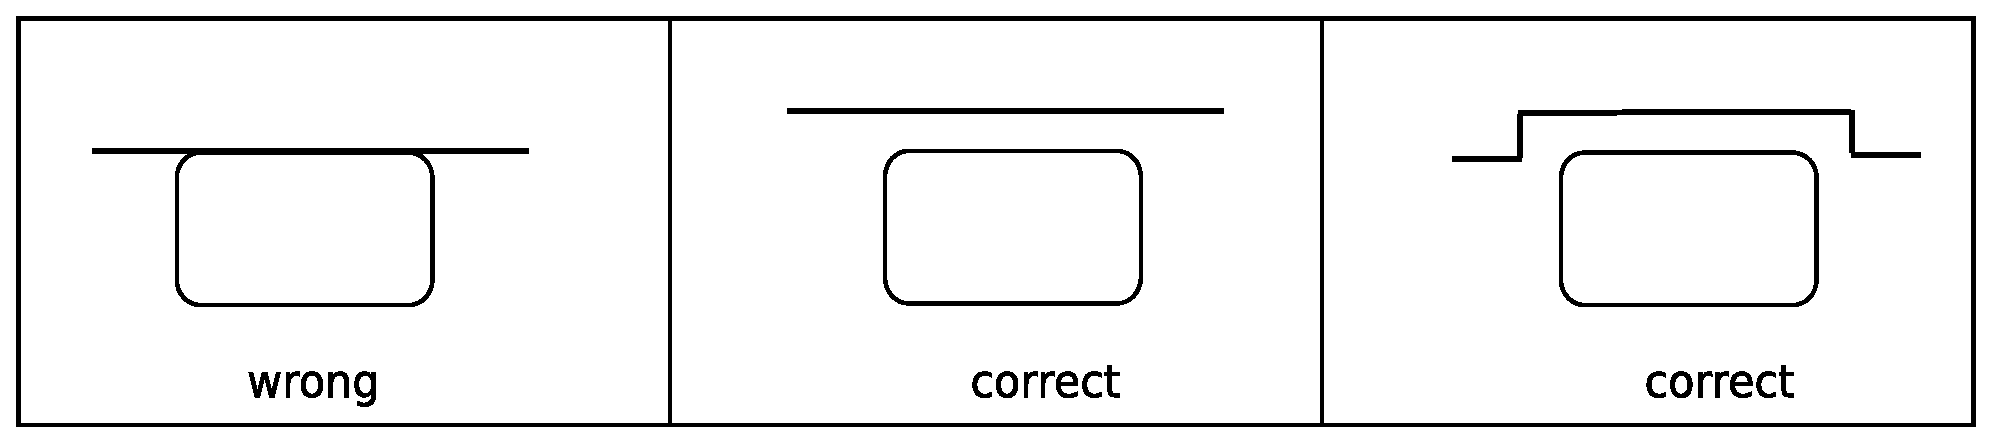
\includegraphics[scale=0.3]{images/layout-node-border-edge}
  \caption{Edges must not overlap node borders.}\label{layout3}
\end{figure}

\subsubsection{Edge-edge overlaps}

Edges are not allowed to overlap. This include touching of edges.
Furthermore, an edge is neither allowed to cross itself nor to cross
a boundary of nodes or other edges more than once.

\begin{figure}[h!]
  \centering
  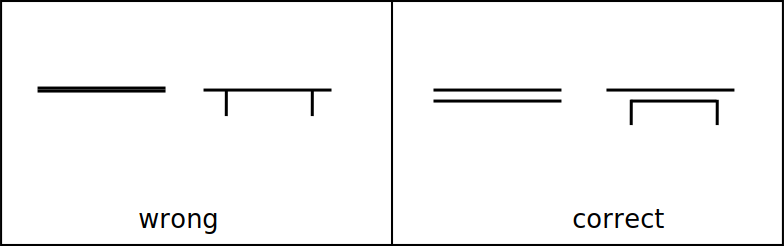
\includegraphics[scale=0.3]{images/layout-edge-edge}
  \caption{Edges must not overlap.}\label{layout4}
\end{figure}

\subsubsection{Node orientation}

Nodes have to be drawn horizontally or vertically, any other
rotation of elements is not allowed.

\begin{figure}[h!]
  \centering
  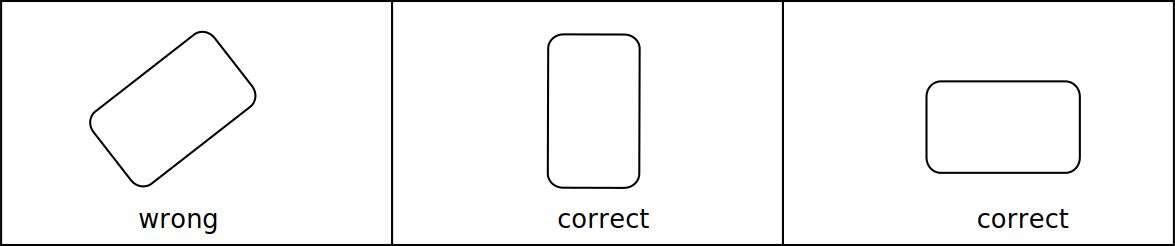
\includegraphics[scale=0.3]{images/layout-orientation}
  \caption{The node orientation must be horizontally or
  vertically.}\label{layout5}
\end{figure}

\subsubsection{Node-edge connection}

The arcs linking the square box of a transition to the state/entity
nodes are attached to the center of opposite sides. The modulatory
arcs point are attached to the other two sides, but not necessarily
all to the center as several modifiers can touch the same transition
node. A transition connected to glyph-production arcs on opposite
sides is a reversible transition.

\begin{figure}[h!]
  \centering
  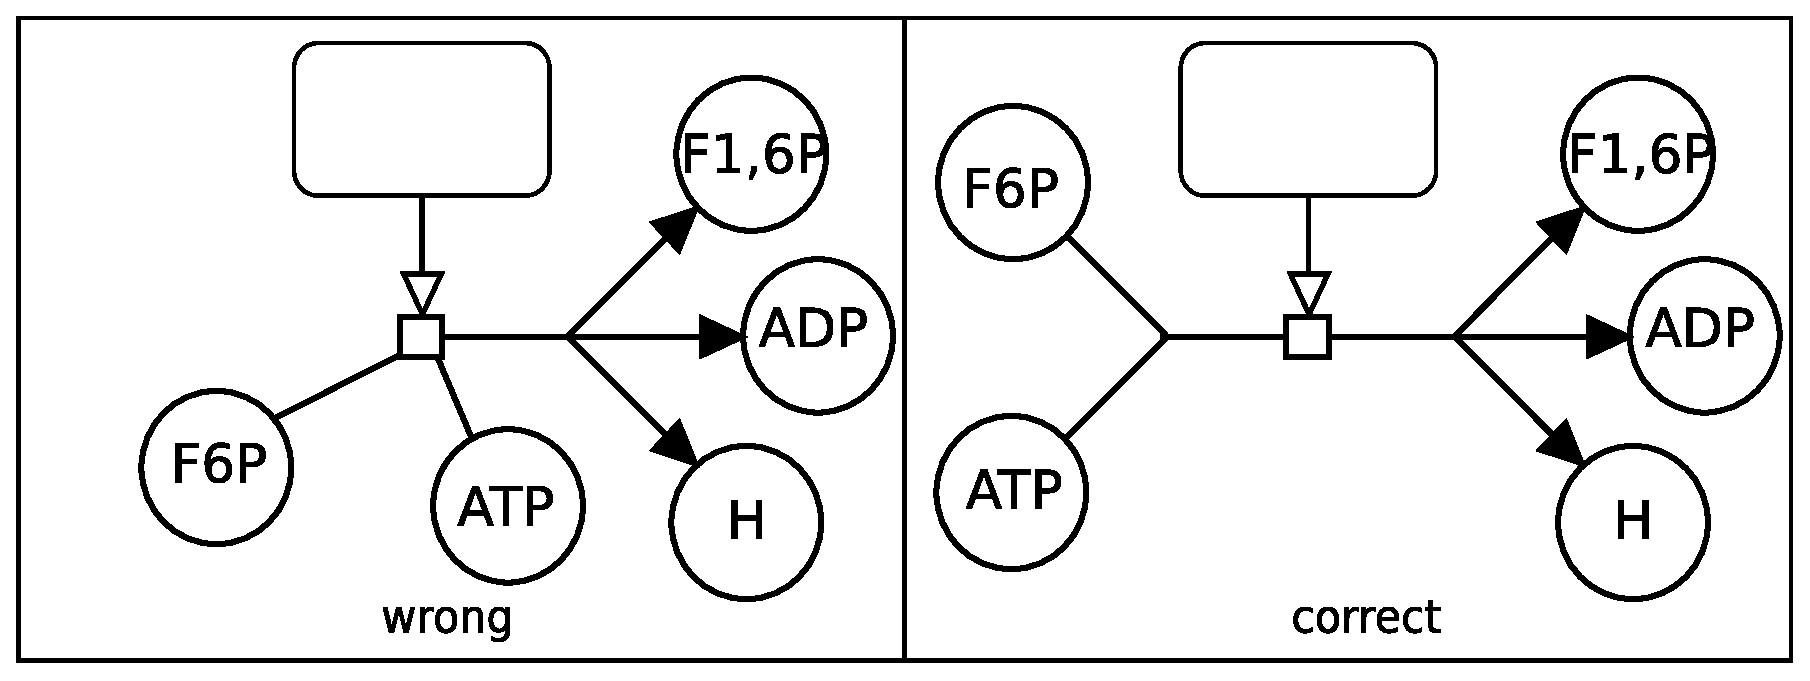
\includegraphics[scale=0.3]{images/layout-connecting-arcs}
  \caption{Arcs between a transition and the state/entity
  nodes must be attached to the center of opposite sides, modulatory
  arcs must be attached to the other two sides.}\label{layout6}
\end{figure}

\subsubsection{Node labels}

At least a part of the label (unbordered box containing a string of
characters) has to be placed inside the node it belongs to. Node
labels are not allowed to overlap nodes or other labels (this
includes touching of other nodes or labels).

\subsubsection{Edge labels}

Edge labels are not allowed to overlap nodes. This includes touching
of nodes.

\subsubsection{Compartments}

If a transition has all participants in the same compartment the
transition node and all edges/arcs have to be in this compartment.
If a transition has participants in at least two different
compartments, the transition node has to be either in a compartment
where the transition has at least one participant or in the empty
space.

\subsubsection{Interaction edge}

Other arcs ending at an interaction edge must end in the interaction
zone. The dots representing the connection of an arc with the
interaction zone should be equally distributed. The interaction zone
consisting of two connected edges is either a circle or an enclosed
area with the two edges parallel.

\newpage
\subsection{Recommendations}

Recommendations are rules which should be followed if possible to
produce layouts which look similar (better formulation) and may be
easier to understand.

\subsubsection{Node-edge crossing}\label{crosEdNo}

Crossings between edges and nodes should be avoided. Some crossings
may be unavoidable, e.\,g.~the crossing between an edge and a
compartment border or an edge and a complex (if the edge connects an
element inside the complex with something outside). See also
requirement \ref{crosEdNoRe} (in case of node-edge crossings the
edge must be drawn on the top of the node).

\subsubsection{Labels}

Labels should be horizontal. Node labels should be placed completely
inside the node if possible. Edge labels should be placed close to
the edge and avoid overlapping the edge as well as other edge
labels.

\subsubsection{Avoid edge crossings}

Crossings between edges should be minimized.

\subsubsection{Units of information}

Units of information should not hide the structure of the
corresponding node.

\begin{figure}[h!]
  \centering
  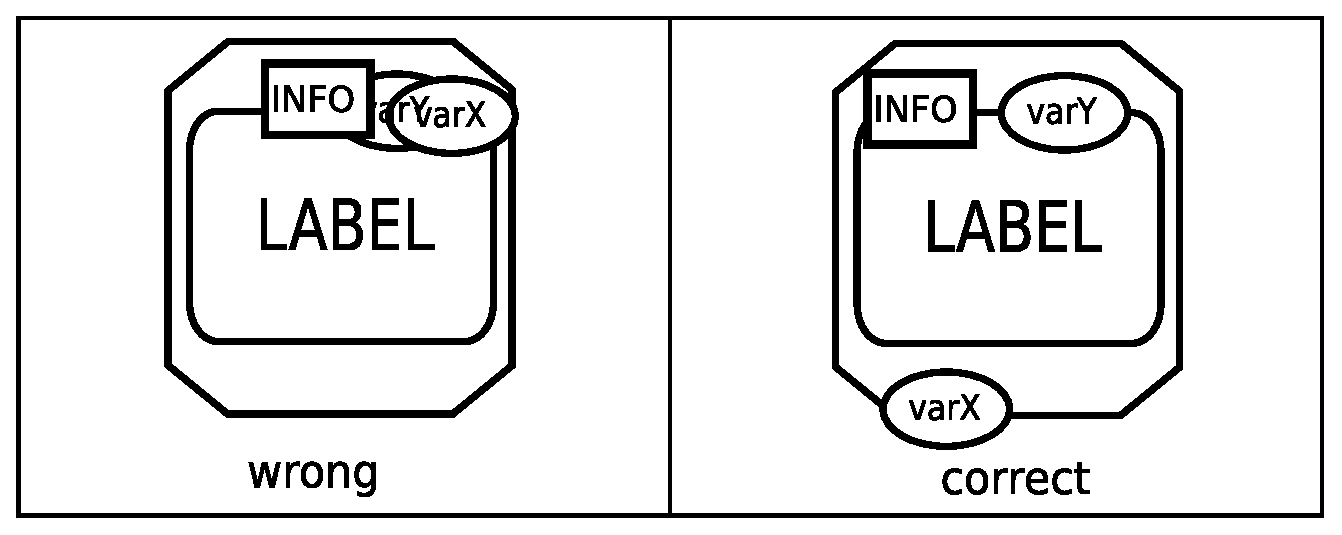
\includegraphics[scale=0.5]{images/layout-unit-information}
  \caption{Units of information should not overlap with any
  other element.}\label{layout7}
\end{figure}

\newpage
\subsection{Additional suggestions}

Here is a list of additional layout suggestions which may help in
producing aesthetically more pleasing layouts which may be easier to
understand.

\begin{itemize}
  \item Angle of edge crossings: If edge crossings are not avoidable
  edges should cross with an angle close to 90 degrees.
  \item Placement of substrates and products of a transition:
  Substrate and product nodes should be placed
  on different sides of the transition node.
  \item Drawing area and width/height ratio: The drawing should
  be compact and the ratio between the width and the height
  of the drawing should be close to 1.
  \item Edge length: Long edges should be avoided and the
  edge length should be minimized.
  \item Number of edge bends: Edges should be drawn with
  as few bends as possible.
  \item Similar and symmetric parts: Similar parts of a diagram
  should be drawn in a similar way, and symmetric parts
  should be drawn symmetrically.
  \item Proximity information: Related elements (e.\,g.~nodes
  connected by a transition or all elements within a compartment)
  should be drawn close together.
  \item Directional information: Subsequent processes (e.\,g.~a sequence
  of reactions) should be drawn in one direction (e.\,g.~from
  top to bottom or from left to right).
  \item Compartments: Different compartments should have different
  background shade or color.
\end{itemize}
